% Options for packages loaded elsewhere
\PassOptionsToPackage{unicode}{hyperref}
\PassOptionsToPackage{hyphens}{url}
%
\documentclass[
]{article}
\title{Does Elon Musk's tweets influence Bitcoin market value? : A
sentiment anaylsis approach}
\author{Beatrice Stocco - Federico Piazza - Luigi Negro}
\date{04/04/2022}

\usepackage{amsmath,amssymb}
\usepackage{lmodern}
\usepackage{iftex}
\ifPDFTeX
  \usepackage[T1]{fontenc}
  \usepackage[utf8]{inputenc}
  \usepackage{textcomp} % provide euro and other symbols
\else % if luatex or xetex
  \usepackage{unicode-math}
  \defaultfontfeatures{Scale=MatchLowercase}
  \defaultfontfeatures[\rmfamily]{Ligatures=TeX,Scale=1}
\fi
% Use upquote if available, for straight quotes in verbatim environments
\IfFileExists{upquote.sty}{\usepackage{upquote}}{}
\IfFileExists{microtype.sty}{% use microtype if available
  \usepackage[]{microtype}
  \UseMicrotypeSet[protrusion]{basicmath} % disable protrusion for tt fonts
}{}
\makeatletter
\@ifundefined{KOMAClassName}{% if non-KOMA class
  \IfFileExists{parskip.sty}{%
    \usepackage{parskip}
  }{% else
    \setlength{\parindent}{0pt}
    \setlength{\parskip}{6pt plus 2pt minus 1pt}}
}{% if KOMA class
  \KOMAoptions{parskip=half}}
\makeatother
\usepackage{xcolor}
\IfFileExists{xurl.sty}{\usepackage{xurl}}{} % add URL line breaks if available
\IfFileExists{bookmark.sty}{\usepackage{bookmark}}{\usepackage{hyperref}}
\hypersetup{
  pdftitle={Does Elon Musk's tweets influence Bitcoin market value? : A sentiment anaylsis approach},
  pdfauthor={Beatrice Stocco - Federico Piazza - Luigi Negro},
  hidelinks,
  pdfcreator={LaTeX via pandoc}}
\urlstyle{same} % disable monospaced font for URLs
\usepackage[margin=1in]{geometry}
\usepackage{color}
\usepackage{fancyvrb}
\newcommand{\VerbBar}{|}
\newcommand{\VERB}{\Verb[commandchars=\\\{\}]}
\DefineVerbatimEnvironment{Highlighting}{Verbatim}{commandchars=\\\{\}}
% Add ',fontsize=\small' for more characters per line
\usepackage{framed}
\definecolor{shadecolor}{RGB}{248,248,248}
\newenvironment{Shaded}{\begin{snugshade}}{\end{snugshade}}
\newcommand{\AlertTok}[1]{\textcolor[rgb]{0.94,0.16,0.16}{#1}}
\newcommand{\AnnotationTok}[1]{\textcolor[rgb]{0.56,0.35,0.01}{\textbf{\textit{#1}}}}
\newcommand{\AttributeTok}[1]{\textcolor[rgb]{0.77,0.63,0.00}{#1}}
\newcommand{\BaseNTok}[1]{\textcolor[rgb]{0.00,0.00,0.81}{#1}}
\newcommand{\BuiltInTok}[1]{#1}
\newcommand{\CharTok}[1]{\textcolor[rgb]{0.31,0.60,0.02}{#1}}
\newcommand{\CommentTok}[1]{\textcolor[rgb]{0.56,0.35,0.01}{\textit{#1}}}
\newcommand{\CommentVarTok}[1]{\textcolor[rgb]{0.56,0.35,0.01}{\textbf{\textit{#1}}}}
\newcommand{\ConstantTok}[1]{\textcolor[rgb]{0.00,0.00,0.00}{#1}}
\newcommand{\ControlFlowTok}[1]{\textcolor[rgb]{0.13,0.29,0.53}{\textbf{#1}}}
\newcommand{\DataTypeTok}[1]{\textcolor[rgb]{0.13,0.29,0.53}{#1}}
\newcommand{\DecValTok}[1]{\textcolor[rgb]{0.00,0.00,0.81}{#1}}
\newcommand{\DocumentationTok}[1]{\textcolor[rgb]{0.56,0.35,0.01}{\textbf{\textit{#1}}}}
\newcommand{\ErrorTok}[1]{\textcolor[rgb]{0.64,0.00,0.00}{\textbf{#1}}}
\newcommand{\ExtensionTok}[1]{#1}
\newcommand{\FloatTok}[1]{\textcolor[rgb]{0.00,0.00,0.81}{#1}}
\newcommand{\FunctionTok}[1]{\textcolor[rgb]{0.00,0.00,0.00}{#1}}
\newcommand{\ImportTok}[1]{#1}
\newcommand{\InformationTok}[1]{\textcolor[rgb]{0.56,0.35,0.01}{\textbf{\textit{#1}}}}
\newcommand{\KeywordTok}[1]{\textcolor[rgb]{0.13,0.29,0.53}{\textbf{#1}}}
\newcommand{\NormalTok}[1]{#1}
\newcommand{\OperatorTok}[1]{\textcolor[rgb]{0.81,0.36,0.00}{\textbf{#1}}}
\newcommand{\OtherTok}[1]{\textcolor[rgb]{0.56,0.35,0.01}{#1}}
\newcommand{\PreprocessorTok}[1]{\textcolor[rgb]{0.56,0.35,0.01}{\textit{#1}}}
\newcommand{\RegionMarkerTok}[1]{#1}
\newcommand{\SpecialCharTok}[1]{\textcolor[rgb]{0.00,0.00,0.00}{#1}}
\newcommand{\SpecialStringTok}[1]{\textcolor[rgb]{0.31,0.60,0.02}{#1}}
\newcommand{\StringTok}[1]{\textcolor[rgb]{0.31,0.60,0.02}{#1}}
\newcommand{\VariableTok}[1]{\textcolor[rgb]{0.00,0.00,0.00}{#1}}
\newcommand{\VerbatimStringTok}[1]{\textcolor[rgb]{0.31,0.60,0.02}{#1}}
\newcommand{\WarningTok}[1]{\textcolor[rgb]{0.56,0.35,0.01}{\textbf{\textit{#1}}}}
\usepackage{graphicx}
\makeatletter
\def\maxwidth{\ifdim\Gin@nat@width>\linewidth\linewidth\else\Gin@nat@width\fi}
\def\maxheight{\ifdim\Gin@nat@height>\textheight\textheight\else\Gin@nat@height\fi}
\makeatother
% Scale images if necessary, so that they will not overflow the page
% margins by default, and it is still possible to overwrite the defaults
% using explicit options in \includegraphics[width, height, ...]{}
\setkeys{Gin}{width=\maxwidth,height=\maxheight,keepaspectratio}
% Set default figure placement to htbp
\makeatletter
\def\fps@figure{htbp}
\makeatother
\setlength{\emergencystretch}{3em} % prevent overfull lines
\providecommand{\tightlist}{%
  \setlength{\itemsep}{0pt}\setlength{\parskip}{0pt}}
\setcounter{secnumdepth}{-\maxdimen} % remove section numbering
\usepackage[nottoc]{tocbibind}
\ifLuaTeX
  \usepackage{selnolig}  % disable illegal ligatures
\fi
\usepackage[]{biblatex}
\addbibresource{./referencesProject\_com.bib}

\begin{document}
\maketitle

\emph{Wordcount as of 26/03}: 5610

\hypertarget{abstract}{%
\section{Abstract}\label{abstract}}

Elon Musk, one of the world's wealthiest people, is regarded as a
technical visionary with a social media following of over 79 million
followers on Twitter. This paper aims at examining how Musk's Twitter
engagement influences short-term cryptocurrency price and volume using
an event study approach. After examining 4787 tweets containing 68676
words, posted from December 2011 to January 2021 we found that Musk is
likely to use positive words in his tweets, with ``trust'' and
``anticipation'' as the most frequent sentiments expressed. This results
are also confirmed by applying the same sentiment approach on a
different temporal subset of Tesla CEO's tweets (starting from January
2020, when Musk's popularity unquestionably gained momentum). However,
we did not find evidence to support linkage between Musk's sentiments
and Bitcoin volatility.

\hypertarget{literature-review}{%
\section{Literature review}\label{literature-review}}

Data and text mining has assumed a critical role in recent years, and
Twitter, thanks to its easily accessible API has played a crucial part.

The first data mining activities were conducted around 2013 with the
scope of highlighting how Twitter played a central role in spreading
awareness after a natural disaster
occured\autocite{gunawongSocialNetworkReactions2013}. Similar analyses
have been performed to forecast political election's
results\autocite{hubertyCanWeVote2015} and are now being applied to the
cryptocurrency and stock markets.

\autocite{noferUsingTwitterPredict_2015} found evidence that
follower-weighted social mood levels can predict share returns, even
though this was not true if simple aggregation of mood states was
performed. Indeed, they hypothesized the reason behind such a behavior
could be explained in light of emotional contagion, according to which
individuals influence each other based on their active network. In
2019\autocite{guInformationalRoleSocial2020a} another research was
conducted in this field and it was observed that relevant information
could be found on Twitter, in particular regarding analyst
recommendation changes, target price changes, quarterly earnings
surprises and IPO opening prices. Besides this conclusion, that was in
line with other papers, they also studied another factor with relevant
implications in terms of stock return quality of predictions.
Specifically, they found that Twitter sentiment analysis constituted a
stronger predictor for smaller firms, i.e.~firms less covered by
analysts. Last but not
least,\textcite{porshnevCouldEmotionalMarkers2016} studied the
contribution of emotional makers to the ARMAX-GARCH model and
demonstrated they provided both a smaller BIC and improved likelihood
function.

\hypertarget{sentiment-analysis}{%
\section{Sentiment analysis}\label{sentiment-analysis}}

Some of the text mining techniques include classification and
clustering, sentiment analysis and natural language processing. The
latter represents a broader technique that performs different types of
analysis, namely summarization, part of speech tagging, text
categorization and sentiment analysis.

Particularly relevant to our research is the latter, as emotions have
been proved to be key drivers in the process of investing. ``Sentiment
analysis is a series of methods, techniques, and tools about detecting
and extracting subjective information, such as opinion and attitudes,
from language.''\autocite{mantylaEvolutionSentimentAnalysis2018} It has
historically focused on polarity, meaning the positivity or negativity
expressed in a text, but is now moving to a more accurate detection of
different emotions (frustration, joy, anger, sadness, excitement).

The first paper using sentiment analysis dates back to 1940, where
opinions on various public issues were investigated. A similar analysis
was performed a couple years later on countries that mostly suffered
during WW2. But it is not until the early 21st century that more and
more papers were published. In 2010 Sitaram Asur and Bernardo A.
Huberman used data from Twitter to build a linear regression model to
predict box-office revenues of movies in advance of their release. The
predictor used was rate of chatter, but they highlighted how a sentiment
analysis improved predictions after a movie was released. In particular,
they constructed a sentiment analysis classifier to distinguish
positive, negative or neutral texts. They then created two factors:
Subjectivity and Polarity. With the first they were able to confirm
their hypothesis, according to which ``there were more sentiments
discovered in tweets for the weeks after release, than in the
pre-release week''. The polarity factor, i.e.~polarity= Tweets with
Positive Sentiment divided by Tweets with Negative Sentiment was used to
correlate positive sentiments with revenue increases.

In 2012 Younggue Bae,Hongchul Lee examined the positive or negative
influence of popular twitterers on the sentiment of audience. They
started out by selecting 13 popular users and for each of them they
identifies their audience, i.e.~those people ``who reply to, mention, or
retweet about the popular
user''.\autocite{baeSentimentAnalysisTwitter2012a} Using lexicon-based
sentiment analysis they were able to divide the audience into two
groups: those who are in favour and those who are against the popular
user. They then proceeded on investigating the relationship between the
user sentiment and his audience one. The results showed a general
positive correlation between the two, meaning that positive Tweets of a
popular user were followed by positive retweets and viceversa. Last but
not least, they investigated the relationship between real-world
landscape and influence of popular users and found a strong casuality
correlation. This too appears to be an important result: Twitter can be
used as a predictor of real world landscape.

\hypertarget{introduction}{%
\section{Introduction}\label{introduction}}

On January 29, 2021, Elon Musk, at that time the richest person in the
world unexpectedly changed the bio1 of his Twitter account to \#bitcoin.
The price of Bitcoin rose from about 32,000\$ to over 38,000\$ in a
matter of hours, increasing the asset's market capitalization by 111
billion \$ The relevance of Musk's tweets for financial markets has
already become apparent in other contexts. Musk's endorsement of the
encrypted messaging service Signal led to investors purchasing the
unrelated Signal Advance stock, increasing the latter's market valuation
from 55\$ million to over 3\$ billion. These events clearly show the
impact that leadership in social networks can have on financial markets
and the decision-making behavior of (individual) investors. While the
market may read Musk's tweets on Tesla as ``true news,'' his tweets
regarding cryptocurrency reflect moods or personal sentiment, which have
been shown to influence financial market pricing
(\autocite{TwitterMoodPredicts}).

Musk's tweets appear to effect the cryptocurrency market, regardless of
whether they are meant in fun or in earnest, which is our incentive to
look into the topic further and analyse its consequences. While Musk is
far from the only public figure to speak out on social media regarding
cryptocurrency or financial markets, he is undoubtedly one of the most
influential. In strategic contacts between prominent individuals such as
managers, journalists, or financial analysts and stakeholder groups,
social media plays a key role \autocite{HowStrategicLeaders}. Strategic
leaders' social media activities, on the other hand, can generate a lot
of ambiguity. For example, it may be difficult to tell whether a message
is simply expressing a mood or conveying specific company-related
information. It could be hard to ascertain whether a message is merely
expressing a mood or conveying specific company-related information.
Furthermore, stakeholders may be overwhelmed with irrelevant information
that diverts their attention away from the main concerns
\autocite{songSentimentAwareContextualModel2021}. Several research have
looked into the relationship between cryptocurrency markets and social
media activity, particularly on Twitter. Short-term Bitcoin liquidity is
increased by an increase in the number of Bitcoin-related tweets
\autocite{FullArticleHow}, the number of Bitcoin-related tweets can
explain Bitcoin trading volume and returns (Philippas et al., 2019; Shen
et al., 2019), and Twitter sentiment can predict cryptocurrency returns
(Philippas et al., 2019). While several studies have looked into the
impact of individual tweets on stock market returns (such as
\autocite{bransHisThumbEffect2020}, relating to stock market-related
tweets by Donald Trump), to our knowledge, very few researchers have
examined into the impact of individual tweets on cryptocurrency returns
and trading volume.

This research seeks to analyse the sentiment of one of the world's most
powerful persons' social media activities and on if and how this affects
cryptocurrency price levels.

\hypertarget{research-questions}{%
\subsection{Research questions}\label{research-questions}}

We raise the following research questions to address the issue of
effciency in cryptocurrency markets and the attention their participants
devote to influencers since Elon Musk and other influential individuals
are likely to continue publicly commenting on cryptocurrency for the
foreseeable future.

\emph{RQ1: DO Elon Musk's cryptocurrency-related tweets sentiments have
an effect on the pricing and trading volume of cryptocurrency?}

The answer to this issue can reveal whether tweets can be considered
quality signals in general or whether the market effects seen were
purely coincidental. Second, the AMH predicts that a cryptocurrency that
is less efficient or liquid will be more affected by Musk's tweets.

\emph{RQ2: Do sentiments and polarity of Musk's cryptocurrency-related
tweets differs by considering different time-frames and currencies?}

By answering these two study questions, we will be able to measure and
better understand the impact of social media influencers on
cryptocurrency markets, as well as draw some implications about how to
interpret future events.

\emph{RQ3: Is there a linkage between changes in trend of Bitcoin prices
and Elon Musk's crypto-related tweets?}

In other words, can an Elon Musks' tweet significantly change the mean
trend of Bitcoin?

\hypertarget{data-and-methods}{%
\section{Data and methods}\label{data-and-methods}}

\hypertarget{popularity-analysis}{%
\subsection{Popularity analysis}\label{popularity-analysis}}

The analysis is based on tweets by Elon Musk (twitter.com/elonmusk)
between Jan 2011 to 2022. A data extraction has been conducted via
python since some of its functions were more suitable for our purposes.
The code used can be seen in the \textbf{Annex} section. Our dataframe
resulted in total of 4787 tweets containing 68676 words over a time-span
of 10 years. As stated in the previous section, popularity and influence
are critical factors to be assessed from market participants in order to
assign a certain degree of reliability to the information they receive.
That's why a first investigation has been conducted in this direction.
Elon Musk's influence has been skyrocketing throughout the years, mainly
due to the achievements linked to his companies (namely Space X and
Tesla) proving wrong many opponents who considered his goals too
ambitious to be reached. We used three proxies to quantify his
popularity: namely, the \emph{numbers of likes}, \emph{number of
replies} and \emph{number of retweets} on Musk's tweets. These variables
has been grouped by year in order to identify the trend clearly.

\hypertarget{crypto-related-tweets}{%
\subsection{Crypto-related tweets}\label{crypto-related-tweets}}

In a second step, a subset of the total population of tweets was made,
in order to extract only tweets containing the word \emph{bitcoin}
\textbf{and} \emph{cypto} so to direct our focus to Musk's influence on
cryptomarkets Bitcoin-related. Exploiting the embedded time-stamp of
these peculiar type of tweets, it could be possible to visualize in time
when his tweets (events of interest) were located in respect to the
Bitcoin market capitalization trend.

\hypertarget{sentiment-analysis-1}{%
\subsection{Sentiment Analysis}\label{sentiment-analysis-1}}

Once obtained these data, they represented the input for our models:
Sentiment Analysis and Polarization analysis were conducted, supported
by wordclouds (in order to determine which were the most tweeted words).
Through score assignment it has been possible to detect which were the
most frequent sentiments in Musks's tweets, as well as the duration of
these emotions. The results obtained through this first model helped us
to understand the gradient of emotions provoked by Tesla CEO's tweets
and therefore assessing those as drivers to his popularity and
eventually his influence on cryptomarkets. This approach has been
applied to a subset of Musk's tweets obtained by the following criteria:
all the tweets starting from January 2020 and not containing the word
\emph{AMP}. We believe that removing the most frequent tweeted word and
looking at a more recent timespan would strengthen our study
highlighting any peculiar differences or similarities among the two
datasets.

\hypertarget{testing-for-stationarity}{%
\subsection{Testing for stationarity}\label{testing-for-stationarity}}

Finally, we wanted to investigate the presence of linkages between Elon
Musk's sentiment and Bitcoin volatility: to do that we dirstly tried to
erase the intrinsic trend of Bitcoin so to be able to find any potential
changepoints in a stationary time-series trajectory. We repeated the
same process for Dogecoin. end.

\textbf{Why is Stationarity Important?}

Stationarity can be defined in precise mathematical terms, but for our
purpose we mean a flat looking series, without trend, constant variance
over time, a constant autocorrelation structure over time and no
periodic fluctuations (seasonality). For data to be stationary, the
statistical properties of a system do not change over time. This does
not mean that the values for each data point have to be the same, but
the overall behavior of the data should remain constant. If the data is
non-stationary (meaning it has a trend), we need to remove it in order
to proceed with the analysis. Various tecniques can be used to solve the
issue of non-stationarity: after some attempts, the most succesful one
has been to rely on the \emph{log difference} of time values in Bitcoin
price.

\hypertarget{from-non-stationarity-to-stationarity}{%
\subsubsection{From non-stationarity to
stationarity}\label{from-non-stationarity-to-stationarity}}

Once obtained significant p-values assessing the non-stationarity of the
selected time series, we try to achieve a stationary trend by doing a
log difference among two subsequent values in the cryptocurrency value
obtaining satisfying results. Eventually, we confront key breaking
points where the average value undergoes a relevant change between two
time points and the timestamp of the crypto-related Musk's tweet in
order to visualize any linkages between the two phoenomena.

\hypertarget{results}{%
\section{Results}\label{results}}

\hypertarget{elon-musks-influence}{%
\subsection{Elon Musk's influence}\label{elon-musks-influence}}

As can be seen in the summary table below, Elon Musk's influnece has
grown widely over the years. In 10 years, \textbf{number of replies} per
tweet has grown up to more than 3 million, \textbf{number of retweets}
up to more than 4 million and \textbf{number of likes} up to the
astonishing numbers of more than 50 million. As of December 31st 2021,
Elon Musk's follower amounted to 71.5 mln, which means a very high
coverage of \(72,2%
\).

We can visually understand the exponential trend in the growing
popularity of Tesla CEO's. It comes as no surprise that when
\emph{``Elon Musk speaks, investors listen''}. His influence derives
from his large audience, prone to process the majority of the
information coming from him as good quality information, influencing
their (financial) decision-making process.

\begin{figure}
\centering
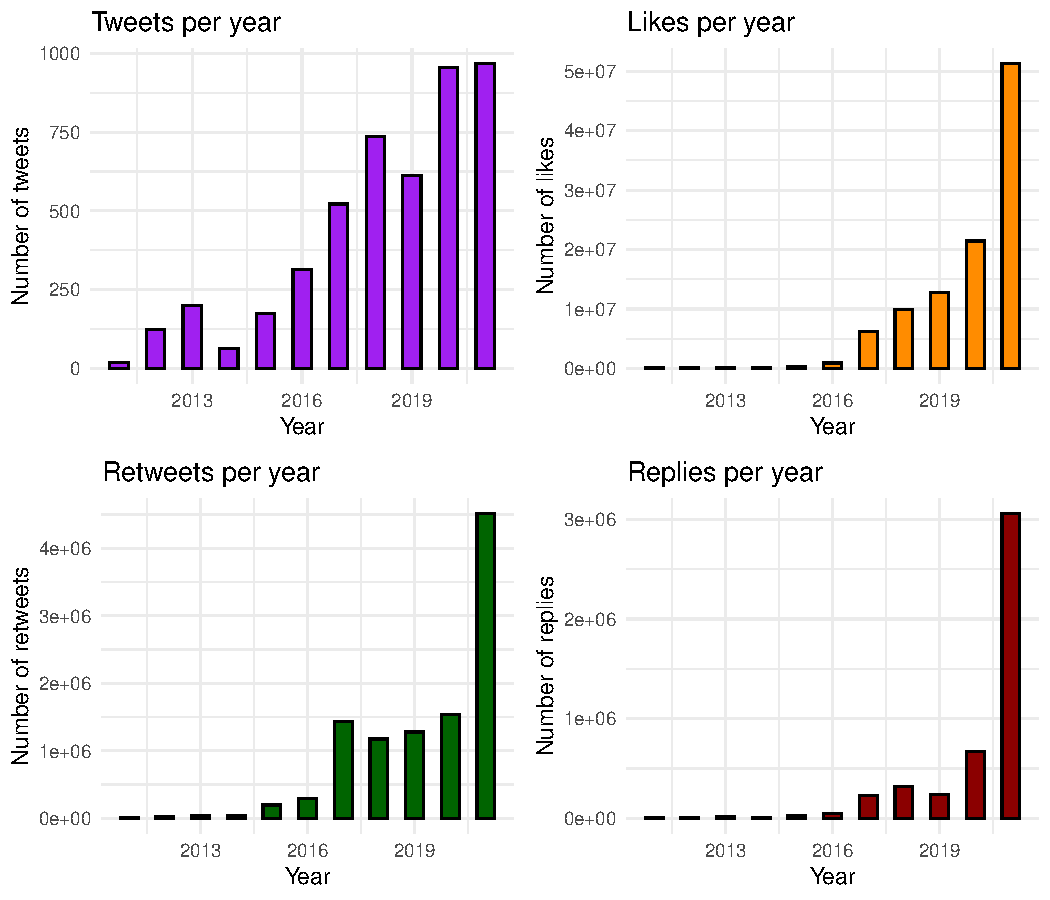
\includegraphics{CopyOfTrial1_files/figure-latex/fi1s-1.pdf}
\caption{\label{fig:fig1}Elon's twitter interaction over time}
\end{figure}

\hypertarget{activty-of-crypto-related-tweets}{%
\subsubsection{Activty of crypto-related
tweets}\label{activty-of-crypto-related-tweets}}

In this section we want to compare how Elon Musk's audience react to
different type of tweets containing respectevely words related only to
\emph{dogecoin}, \emph{Bitcoin} and \emph{cypto}. As in the first
section, we use the \emph{number of likes}, \emph{number of retweets}
and \emph{number of replies} as proxy to popularity and high network
activity more generally. The first two categories are the most popular,
and between the two BTC-related tweets generate slightly more
interaction, coherently with the central importance that Bitcoin has in
the crypto scenario.

\begin{figure}
\centering
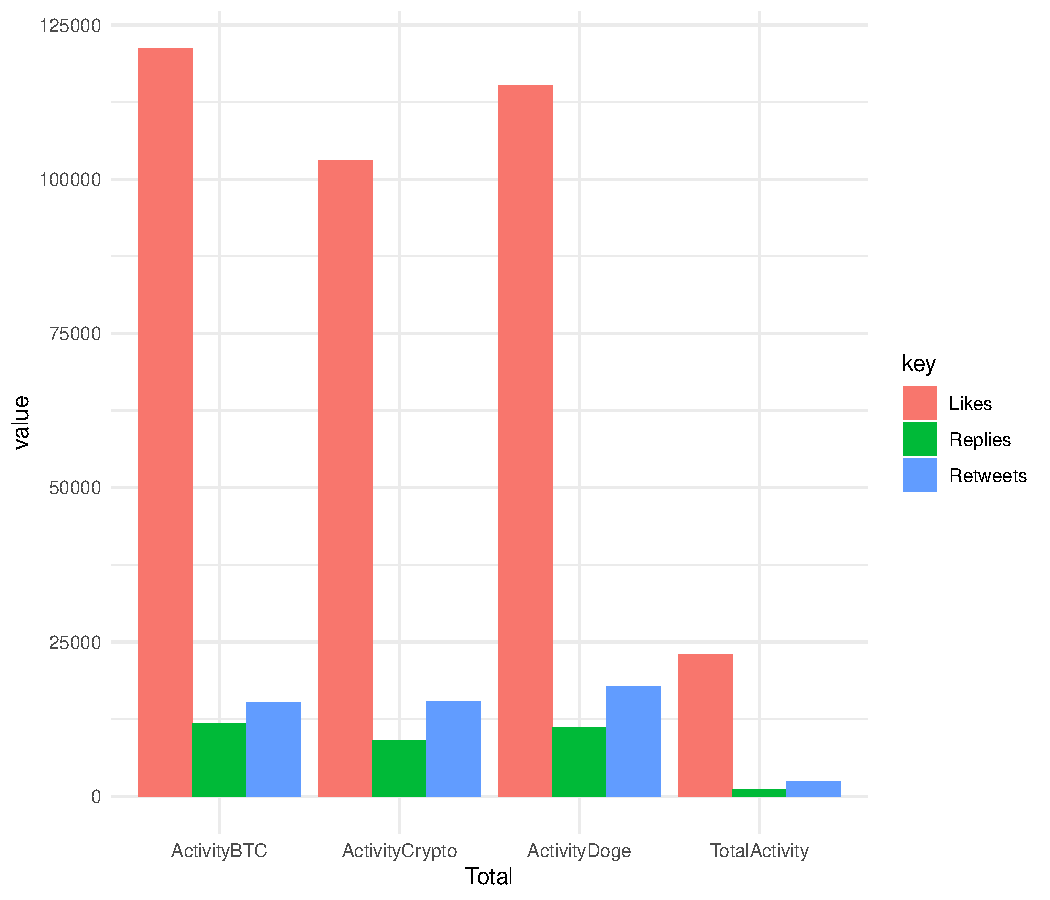
\includegraphics{CopyOfTrial1_files/figure-latex/fig2-1.pdf}
\caption{\label{fig:fig2}Crypto-related content interaction}
\end{figure}

\hypertarget{sentiment-analysis-model-i}{%
\subsection{Sentiment Analysis : Model
I}\label{sentiment-analysis-model-i}}

While the market may interpret Musk's tweets about Tesla as ``accurate
news'', his tweets about cryptocurrency at least to some degree
represent moods or personal sentiment. In this section we want to
further analyze the nature of this sentiments, the most frequent words
and the emotions associated to them.

The graph below shows the most used word and their frequency. It appears
that the three most used words are \emph{amp}, \emph{tesla} and
\emph{will}. We find the presence of more than 600 words for the firsts
two, while more than 500 words for the latter. It goes without saying
that we expected \textbf{tesla} to be one of the most frequent word in
Musk's tweet, and our interpretation of the word \textbf{will} lies in
that this verb shows his strong willingness and decisive, goal-oriented
character as well as his inclination towards the future sustained by
visionary statements. It can be less clear why \textbf{amp} is among the
most frequent word, therefore we opted for a further explanation.

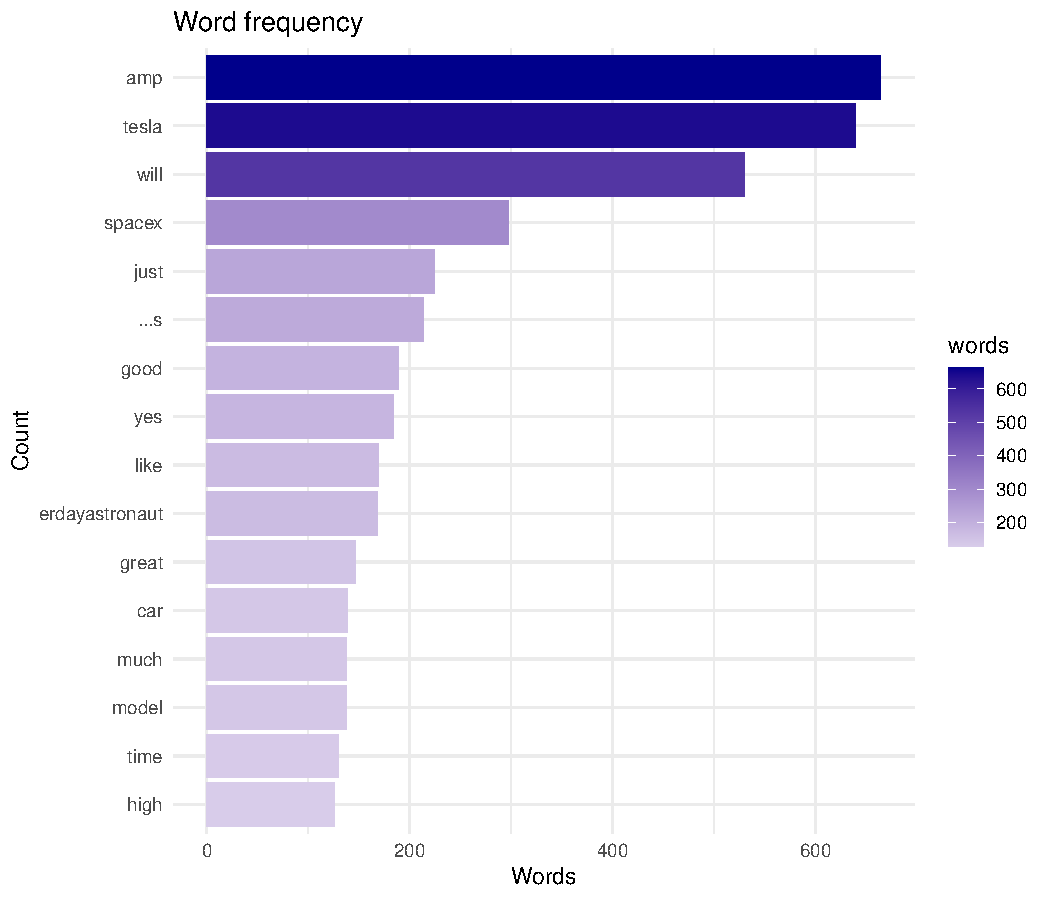
\includegraphics{CopyOfTrial1_files/figure-latex/fig4-1.pdf} \emph{AMP}

Amp is a universal collateral token designed to facilitate fast and
efficient transfers for any real-world application. When using Amp as
collateral, transfers of value are guaranteed and can settle instantly.
While the underlying asset reaches final settlement, a process that can
take anywhere from seconds to days, Amp is held in escrow by a
collateral manager. Once the transaction successfully settles, the Amp
collateral is released and made available to collateralize another
transfer. Amp exists to serve as universal collateral for anyone and any
project. (\emph{Source {[}(\url{https://docs.amptoken.org/}){]}} ).
Besides being a collateral for individuals and DeFi platforms, Amp is
used as a collateral for payment networks: Flexa uses Amp to enable
instant, fraud-free payments to merchants across its digital payment
network. Apps that integrate Flexa stake Amp to ensure all payments can
be settled in real-time regardless of the asset or protocol used. Since
AMP Token was to be integrated with Tesla's payment rail for crypto, it
is understandable why it's been one of the most tweeted words by Elon
Musk, being this news shocking the crypto-lovers panorama and the future
of Tesla. The news of Tesla about the willing to accept crypto as
payments and the investment in over 1.5 BLN USD in Bitcoin (February
2021), made the price of Bitcoin to skyrocket. On the other hand, a
plethora of enviromental activists opposed this decision due to the high
levels of electric energy which are used to mine and sustain the crypto
network and highlighted the controversial nature of the Tesla CEO's
choice: this led Elon Musk to no longer accept payments in Bitcoin. The
impact on the crypto-currency value has been devastating has shown in
the following graphic showing once again, how much ``investors listen to
Elon Musk''.

Here follows a wordcloud which helped us to visualize the most frequent
words in Elon Musk's tweets. The higher the word's size displayed, the
most frequent the word would appear in his tweets.

\hypertarget{sentiment-scores-and-density}{%
\subsubsection{Sentiment scores and
density}\label{sentiment-scores-and-density}}

Based on the following results of the Sentiment Analysis of Elon Musk's
tweets, it appears clear that \emph{positive}, \emph{trust} and
\emph{anticipation} are the most frequent emotions. This result is
perfectly coherent with the visionary Tesla and SpaceX CEO's
personality: his hunger for innovative , out-of-the-box solutions; his
continuous positive and confident approach towards insurmountable
problems such as ``taking the human race to Mars'', conceiving re-usable
rockets disrupting space industry, as well as ``changing the world's
concept of driving through electric autonomous driven vehicle'' and many
others clearly embeds those emotions.

\begin{verbatim}
##   anger anticipation disgust fear joy sadness surprise trust negative positive
## 1     2            1       1    2   1       1        1     1        2        1
## 2     0            0       0    0   0       0        0     0        0        1
## 3     1            1       2    2   0       2        0     1        2        1
## 4     0            0       0    0   0       0        0     1        0        1
## 5     0            1       0    0   1       0        0     3        0        3
## 6     0            0       0    0   0       0        0     0        0        0
\end{verbatim}

\begin{figure}
\centering
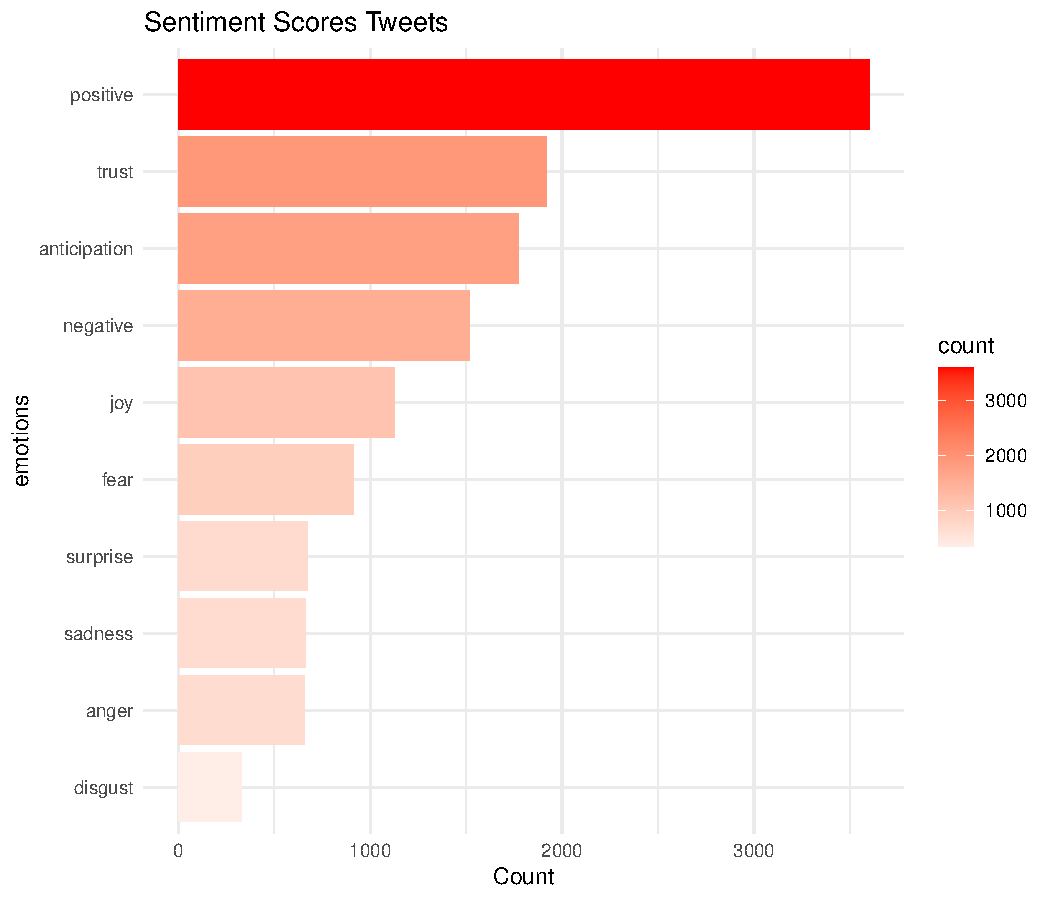
\includegraphics{CopyOfTrial1_files/figure-latex/fig6-1.pdf}
\caption{\label{fig:fig6}Sentiment scores of Elon's tweets}
\end{figure}

Another important result is outlined by the following graphs. It shows
the density of sentiment: as it can be noticed it follows a normal-like
distribution (\(\mu = 0.18\), \$\sigma = 0.36 \$), slightly positevely
skewed. This result is line with the previous results, highlighting the
positive polarity of the sentiments. Here follows a brief statistical
summary of the density plot, followed by the plot itself.

\begin{verbatim}
##          Statistical summary sentiment
## Mean                        0.18242245
## Sd                          0.35932881
## IQR                         0.45907962
## Skewness                   -0.04752713
## Kurtosis                    0.79887814
\end{verbatim}

\begin{figure}
\centering
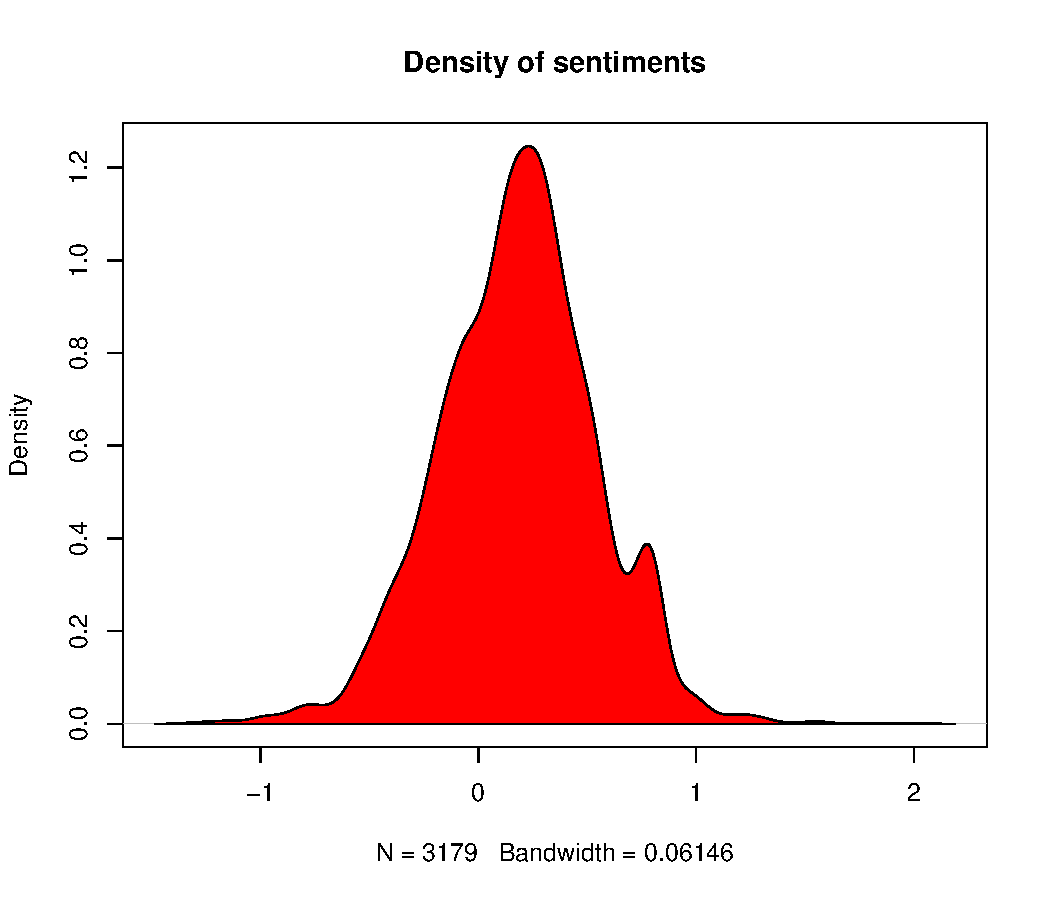
\includegraphics{CopyOfTrial1_files/figure-latex/fig7-1.pdf}
\caption{\label{fig:fig7}density of polarity scores}
\end{figure}

\hypertarget{emotions-at-the-sentence-level}{%
\subsubsection{Emotions at the sentence
level}\label{emotions-at-the-sentence-level}}

The following analysis detects the rate of emotion at the sentence
level. This method uses a simple dictionary lookup to find emotion words
and then compute the rate per sentence. The emotion score ranges between
0 (no emotion used) and 1 (all words used were emotional). Once again,
this result is in line with the previous ones, showing how positive
emotions such as joy, trust and anticipation are predominant. Please
note that the suffix *\_negated* indicates the opposite of the reference
emotions, which appears to be consistently absent in relation to any
emotion.

\begin{figure}
\centering
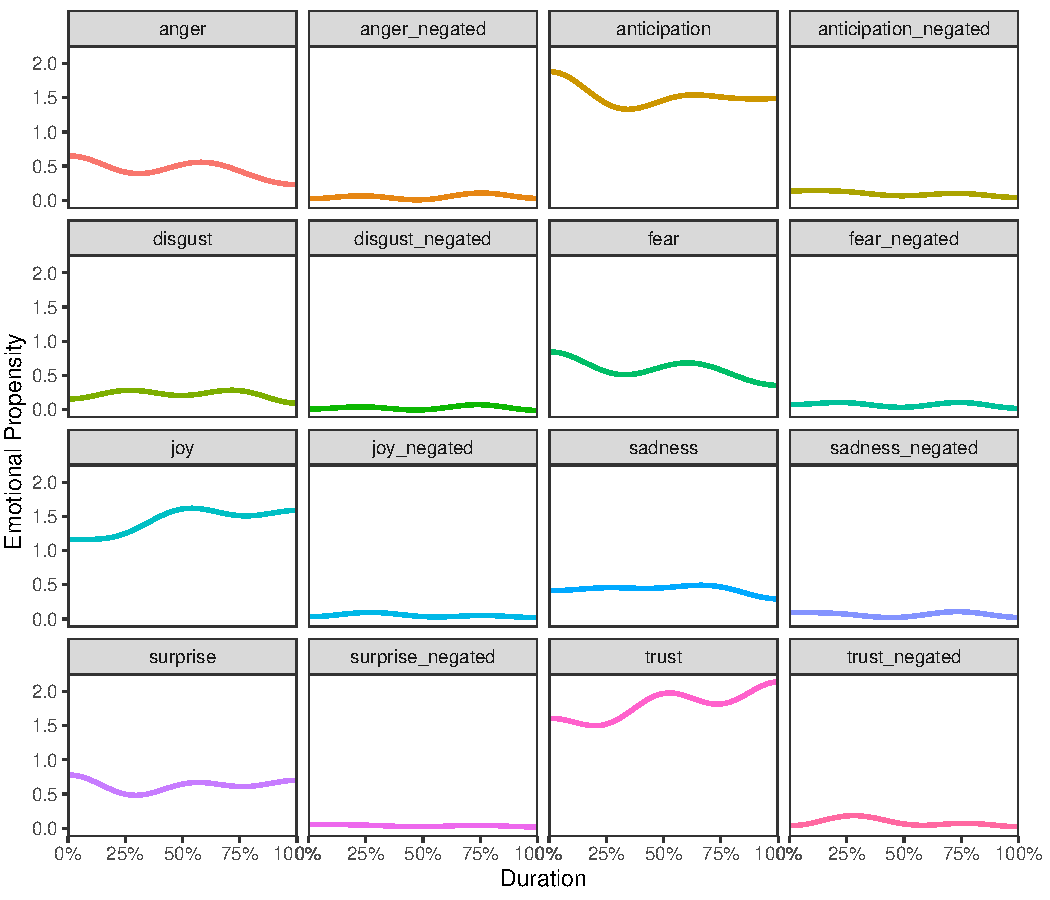
\includegraphics{CopyOfTrial1_files/figure-latex/fig8-1.pdf}
\caption{\label{fig:fig8}plot of Emotions}
\end{figure}

\hypertarget{subsetting-sentiment-from-jan-2020-without-amp-word-sentiment-model-ii}{%
\subsection{Subsetting sentiment from Jan 2020 without ``AMP'' word:
Sentiment model
II}\label{subsetting-sentiment-from-jan-2020-without-amp-word-sentiment-model-ii}}

Once obtained solid result for the entire dataset of tweets ranging from
year 2011 to 2021, it is interesting to compare those with new results
coming from a subset of the selected time frame. We believe it is an
interesting way to assess our results' coherence and a further
investigation into the ``popular'' period of Elon Musk. Furthermore we
believe the most used word, i.e \emph{AMP}, should be removed in order
to assess whether the absence of this word could influence the final
output. In a programatic approach, we apply the same methods, codes and
considerations of the previous section on a different subset of data.

This primary result is in line with the previous ones, once again the
two most used words are \emph{tesla}, \emph{will} and \emph{spacex}. The
frequency of each word is compared in the chart above. We proceed
displaying a wordcloud, in order to have an eye-friendly visualization
of the word frequency in this new subset of data.

\begin{figure}
\centering
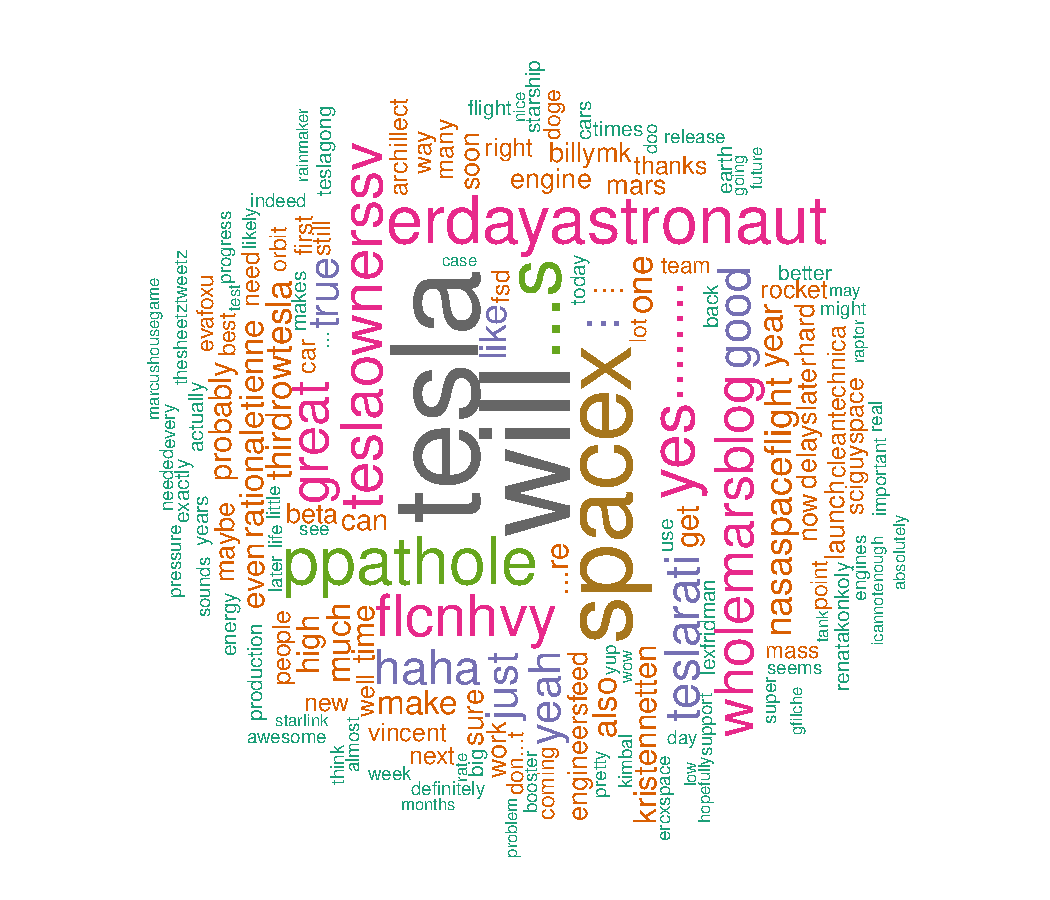
\includegraphics{CopyOfTrial1_files/figure-latex/fig10-1.pdf}
\caption{\label{fig:fig10}Wordcloud of Elon's tweets resampled}
\end{figure}

\hypertarget{sentiment-scores-and-density-1}{%
\subsubsection{Sentiment scores and
density}\label{sentiment-scores-and-density-1}}

Consistently with the previous results, the \emph{Muskanian} influence
is still positive with the most frequent sentiments of \emph{positive},
\emph{anticipation} and \emph{trust}.

The density of sentiment is slightly different from the first one: as it
can be noticed it still follows a normal-like distribution
(\(\mu = 0.19\), \$\sigma = 0.39 \$), slightly positevely skewed. This
result is line with the previous results, stating the even more positive
polarity of the sentiments in the new timeframe. A brief statistical
summary of the new density plot compared to the previous one is
displayed. A new density plot can be found in the chart below.

\begin{verbatim}
## New names:
## * `Statistical summary sentiment` -> `Statistical summary sentiment...1`
## * `Statistical summary sentiment` -> `Statistical summary sentiment...2`
\end{verbatim}

\begin{verbatim}
##          Sentiment model I Sentiment model II
## Mean             0.1981359         0.18242245
## Sd               0.3859845         0.35932881
## IQR              0.5028519         0.45907962
## Skewness        -0.1307537        -0.04752713
## Kurtosis         0.6063917         0.79887814
\end{verbatim}

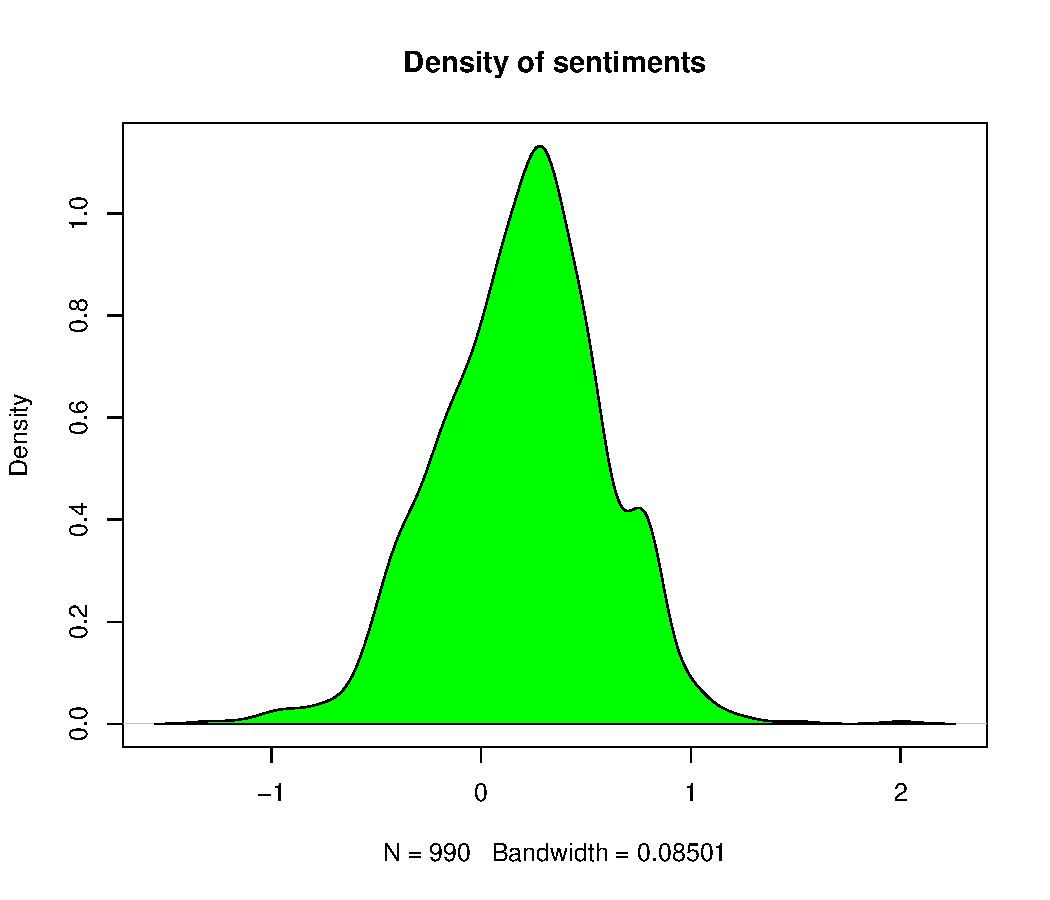
\includegraphics{CopyOfTrial1_files/figure-latex/fig12-1.pdf} The chart
below shows an overall overlapping with the previous result. Still
positive sentiment of \emph{anticipation}, \emph{joy} and \emph{trust}
are the most frequent. However, the sentiment of \emph{trust} is more
volatile, and there is a slight decrease in the negative sentiment of
\emph{fear}. This slight but still relevant change can be interpreted in
a different context than the one of model I: the audience has become
more educated and informed about the phenomenon of crypto-currencies as
well as more critical towards the Tesla CEO's tweets, who sometimes has
been accused more intensively of market manipulation (however without
losing popularity or positive appeal). In conclusion, the Muskanian
audience still listen to him and trust him, simply with more critical
sense which makes the \emph{trust} sentiment to be more volatile and the
\emph{fear} sentiment lower.

\begin{figure}
\centering
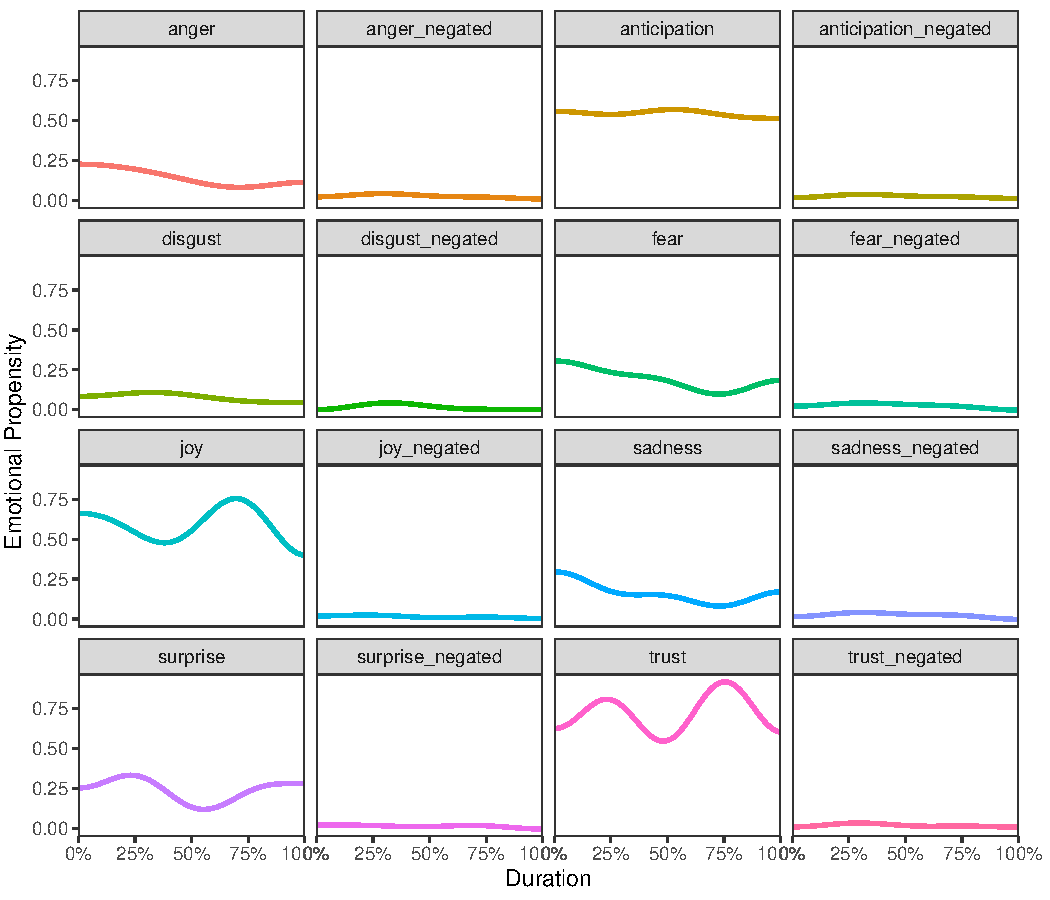
\includegraphics{CopyOfTrial1_files/figure-latex/fig13-1.pdf}
\caption{\label{fig:fig13}Emotion's Plot of Elon's tweets resampled}
\end{figure}

\hypertarget{testing-for-stationarity-1}{%
\subsection{Testing for stationarity}\label{testing-for-stationarity-1}}

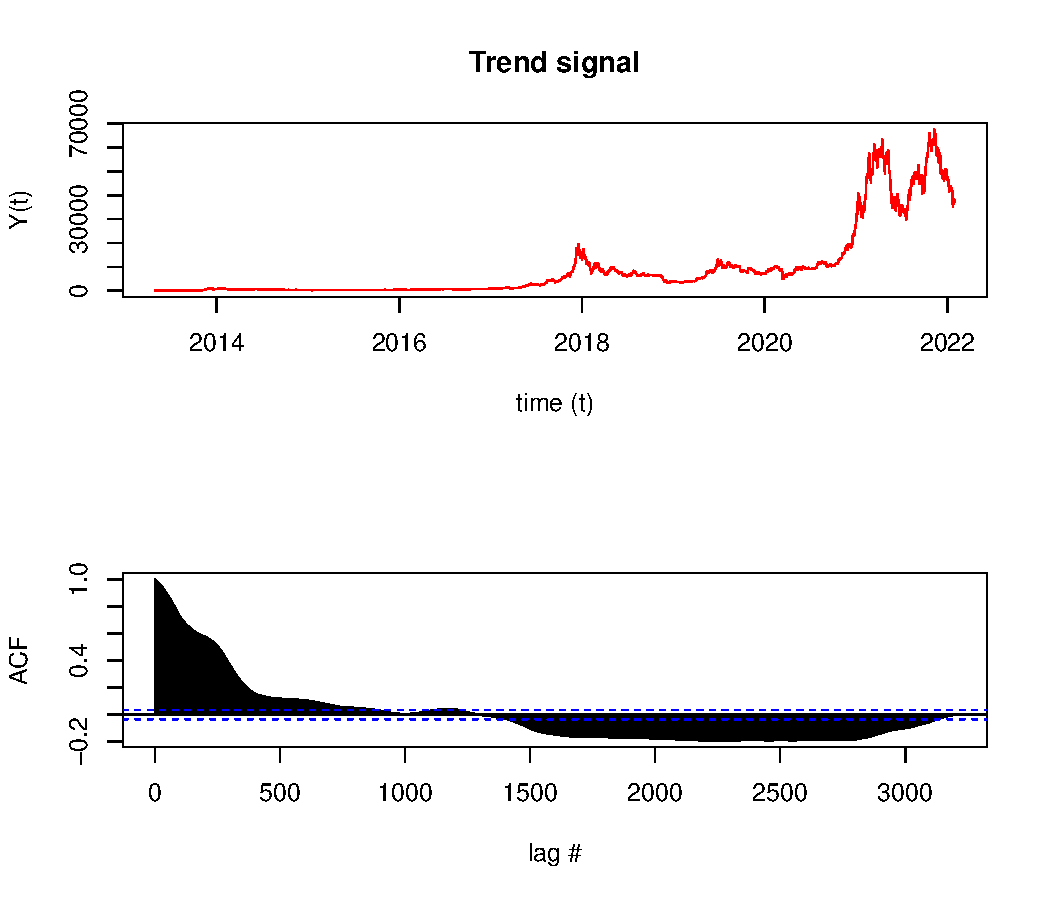
\includegraphics{CopyOfTrial1_files/figure-latex/fig14-1.pdf} We applied
an Augmented Dickey--Fuller (ADF) t-statistic test for unit root: in
statistics and econometrics, an augmented Dickey--Fuller test (ADF)
tests the null hypothesis that a unit root is present in a time series
sample. The alternative hypothesis is different depending on which
version of the test is used, but is usually stationarity or
trend-stationarity. It is an augmented version of the Dickey--Fuller
test for a larger and more complicated set of time series models. The
augmented Dickey--Fuller (ADF) statistic, used in the test, is a
negative number. The more negative it is, the stronger the rejection of
the hypothesis that there is a unit root at some level of confidence.
Our result clearly shows a non-stationarity due to the high p-value
(\textgreater0.5).

\begin{figure}
\centering
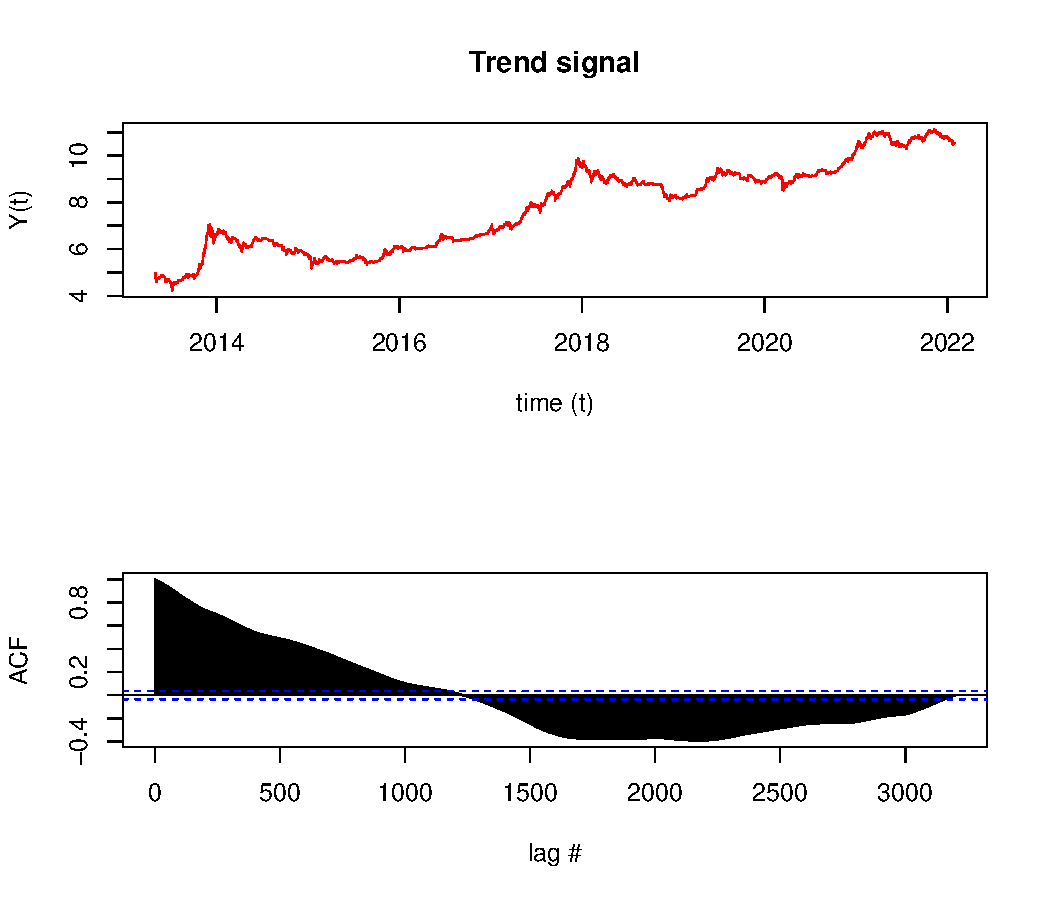
\includegraphics{CopyOfTrial1_files/figure-latex/fig15-1.pdf}
\caption{\label{fig:fig15}LogBitcoin's trend and ACF function}
\end{figure}

Differencing log values can help stabilise the mean of a time series by
removing changes in the level of a time series, and therefore
eliminating (or reducing) trend and seasonality. We attempt to use this
transformation obtaining satisfing results. Indeed, the following plot
shows how the trend has been removed and stationarity is obtained.

\begin{figure}
\centering
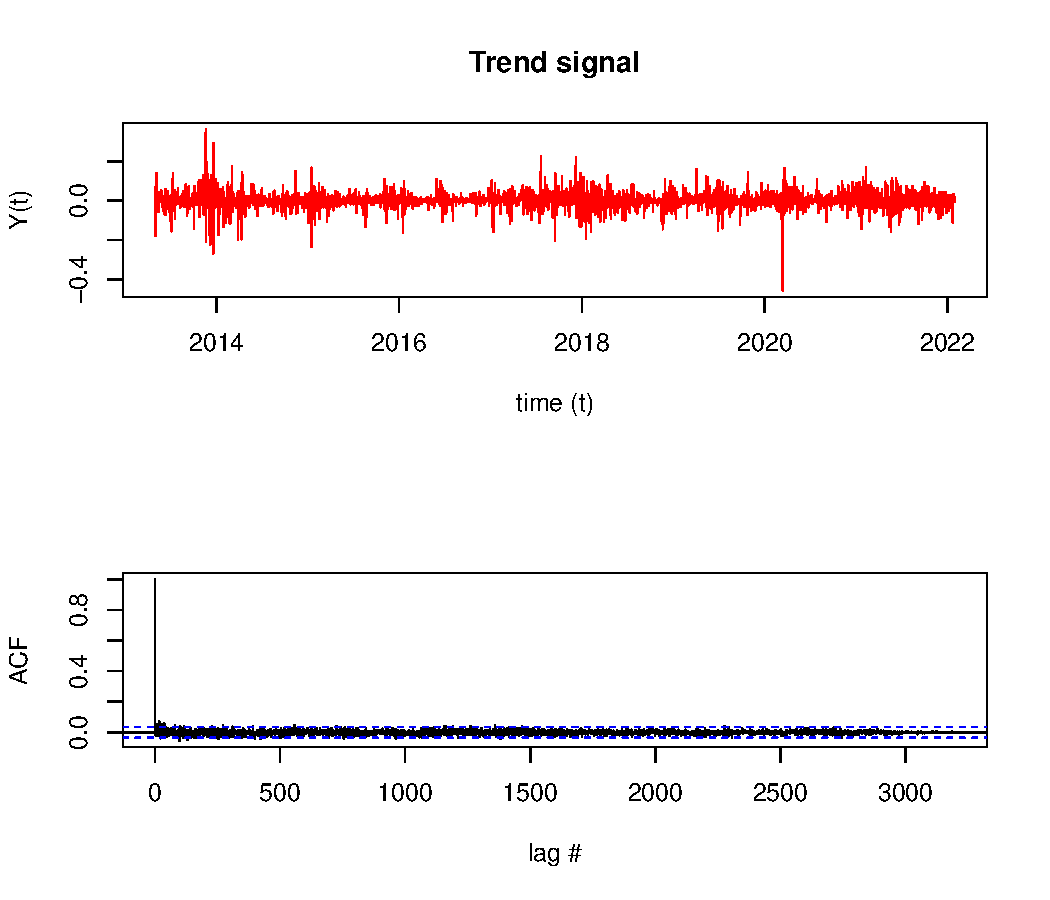
\includegraphics{CopyOfTrial1_files/figure-latex/fig16-1.pdf}
\caption{\label{fig:fig16}Differences of LogBitcoin's trend and ACF
function}
\end{figure}

By being able to use a time-series without stationarity, it might be
possible through some techniques to further investigate if, in a
time-series trajectory with no trend, there are some specific changes in
mean in specific timestamps. To do that we try to identify ``change
points'' in our data. By doing taht we obtain a set of timestamps from
which the variance of the time-series trajectory
changed.\autocite{SurveyMethodsTime} By obtaining those timestamps and
confront it with elon musks' tweet regardind crypto, it is possible to
try to assess whether there is any linkage between the two.

\begin{Shaded}
\begin{Highlighting}[]
\NormalTok{m\_binseg }\OtherTok{\textless{}{-}} \FunctionTok{cpt.mean}\NormalTok{(logdiff, }\AttributeTok{penalty =} \StringTok{"BIC"}\NormalTok{, }\AttributeTok{method =} \StringTok{"BinSeg"}\NormalTok{, }\AttributeTok{Q =} \DecValTok{15}\NormalTok{)}

\FunctionTok{plot}\NormalTok{(m\_binseg, }\AttributeTok{type =} \StringTok{"l"}\NormalTok{, }\AttributeTok{xlab =} \StringTok{"Index"}\NormalTok{, }\AttributeTok{cpt.width =} \DecValTok{4}\NormalTok{)}
\end{Highlighting}
\end{Shaded}

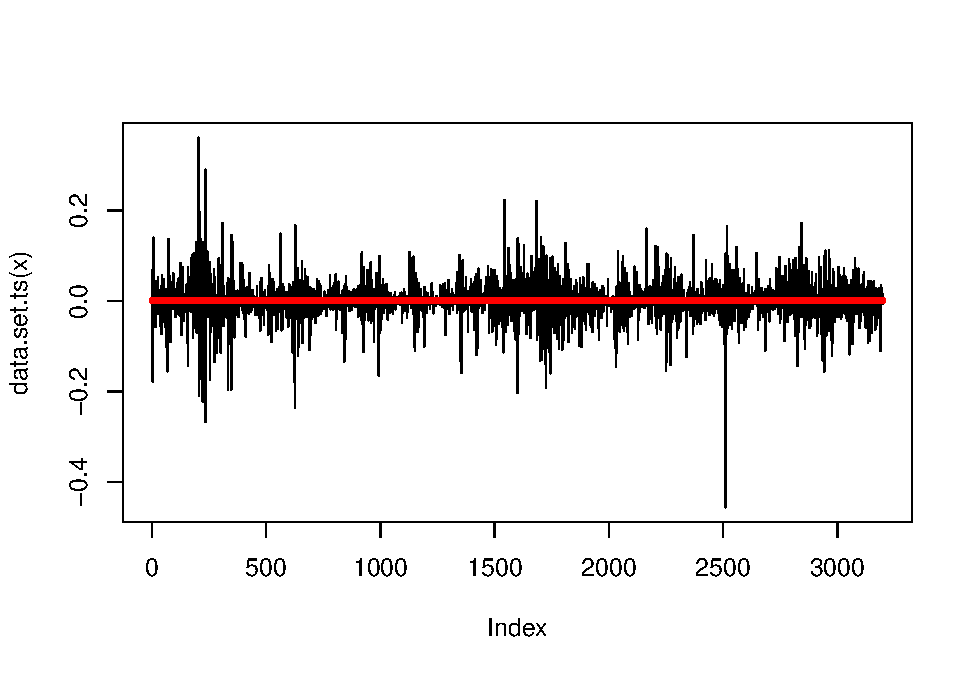
\includegraphics{CopyOfTrial1_files/figure-latex/include==FALSE-1.pdf}

\begin{Shaded}
\begin{Highlighting}[]
\CommentTok{\#all the changes happen from 2750 onwards approx, try to subset plot}
\NormalTok{m\_binseg }\OtherTok{\textless{}{-}} \FunctionTok{cpt.mean}\NormalTok{(logdiff[}\DecValTok{2750}\SpecialCharTok{:}\DecValTok{3199}\NormalTok{], }\AttributeTok{penalty =} \StringTok{"None"}\NormalTok{, }\AttributeTok{method =} \StringTok{"BinSeg"}\NormalTok{, }\AttributeTok{Q =} \DecValTok{15}\NormalTok{)}
\end{Highlighting}
\end{Shaded}

\begin{figure}
\centering
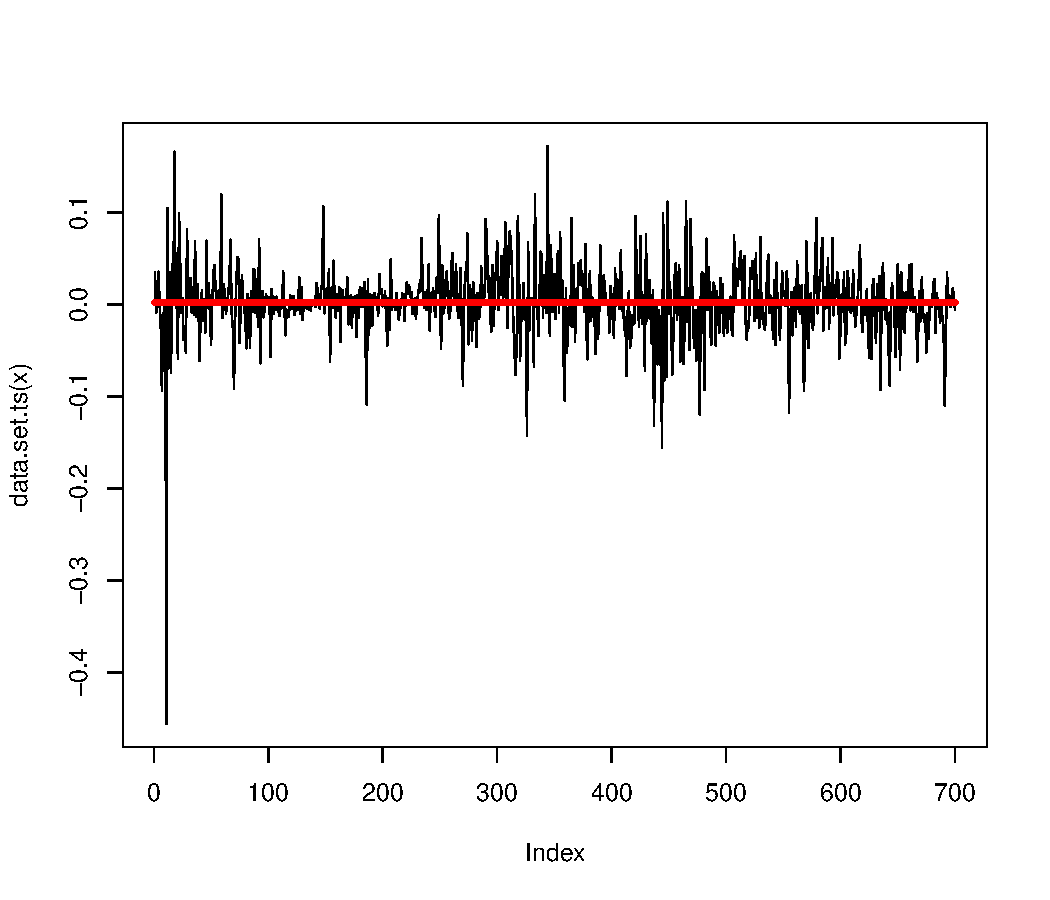
\includegraphics{CopyOfTrial1_files/figure-latex/fig17-1.pdf}
\caption{\label{fig:fig17}Changepoints in LogBitcoin Differences}
\end{figure}

In the chart below a deep investigation regarding the potential linkage
between Bitcoin volatility and Musk's tweet has been conducted. In blue
the \emph{breaking points} are highlighted, which are points in time
where the mean a variable undergoes a significant change. The breaking
points method is broadly used in literature and comprises a variety of
different methods. In purple we find highlighted when the crypto-related
\emph{tweets} were published. As we can notice, there is no
correspondence or correlation of the two variables: we cannot state that
Musk's tweets influence Bitcoin volatility, which is in-line with our
previous result of non-stationarity.

\begin{figure}
\centering
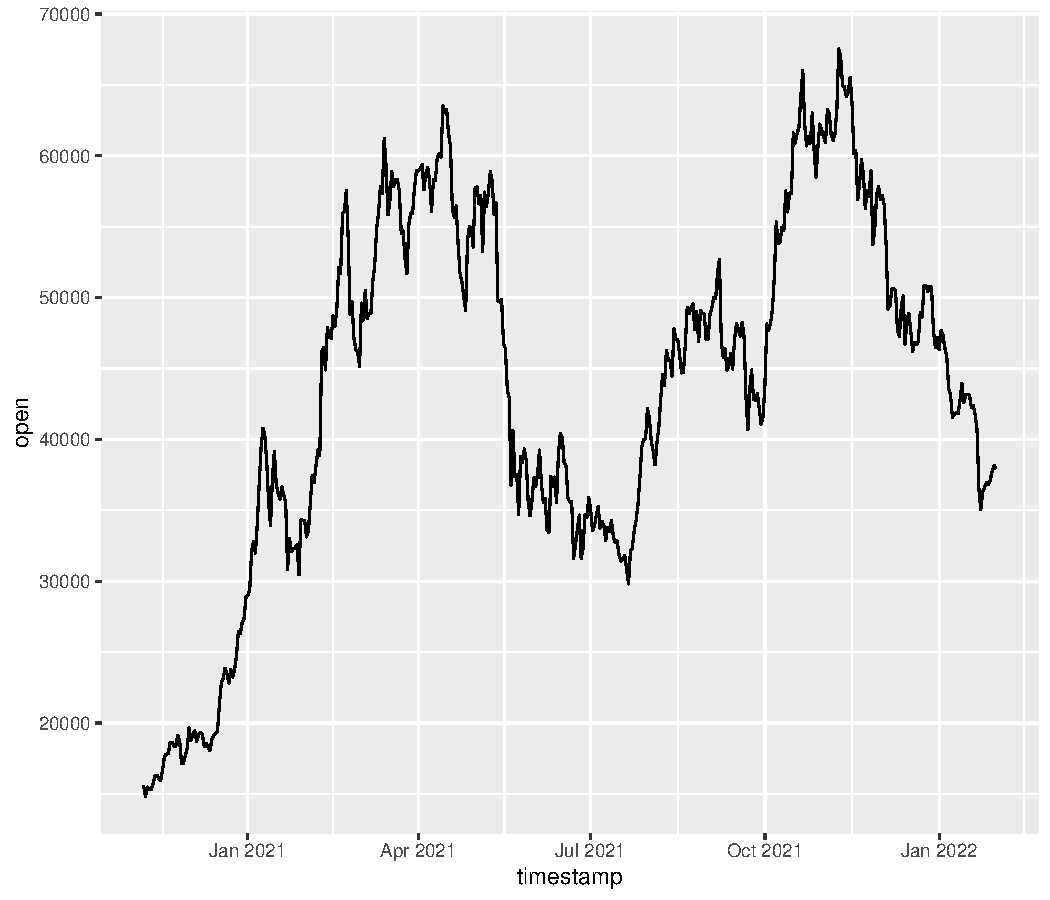
\includegraphics{CopyOfTrial1_files/figure-latex/fig25-1.pdf}
\caption{\label{fig:fig25}Elon Musk's Tweets on Cryptos and LogBTC's
Changing Points Dates}
\end{figure}

Our findings are strenghtened by the confirming the previous result and
considerations for the Dogecoin cryptocurrency. We proceed in the same
way as before, analzying the trend signal and moving from
non-stationarity towards stationarity, as it can be seen in the results
below.

\begin{figure}
\centering
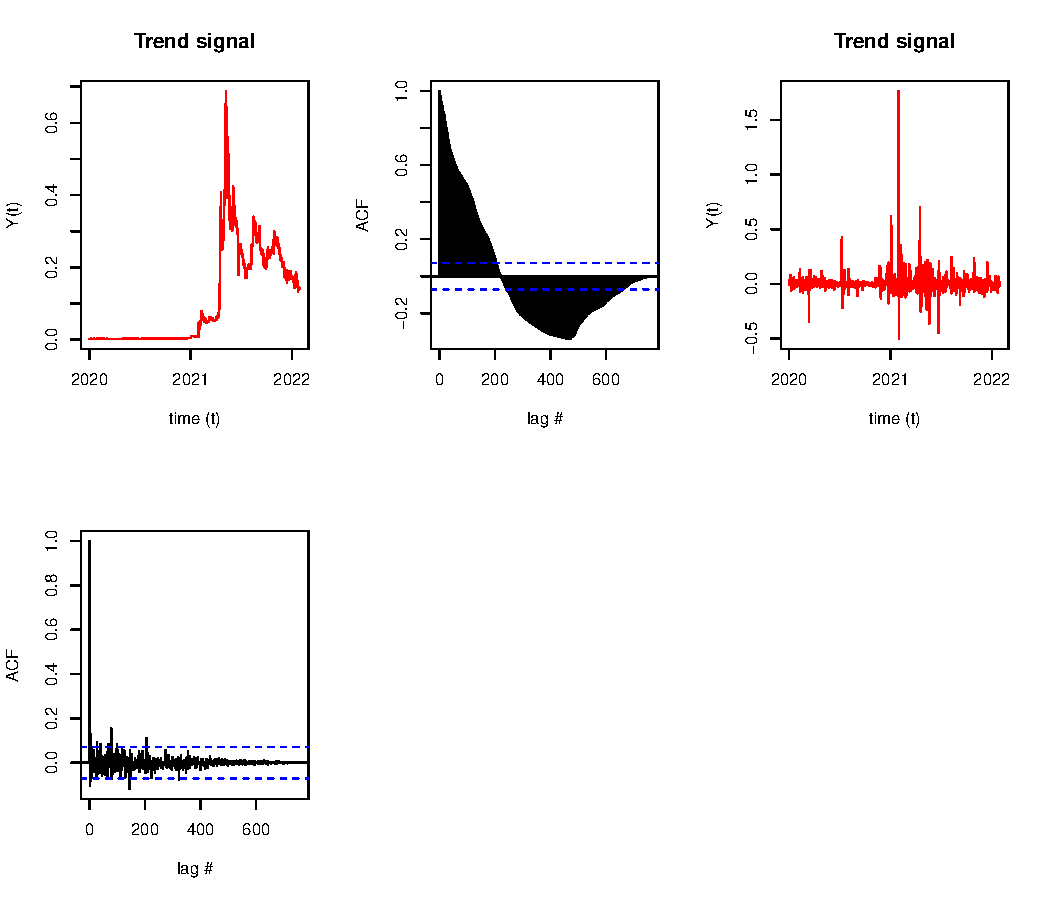
\includegraphics{CopyOfTrial1_files/figure-latex/fig19-1.pdf}
\caption{\label{fig:fig19}Doge and Diff LogDoge trend with its
respective ACF}
\end{figure}

\begin{figure}
\centering
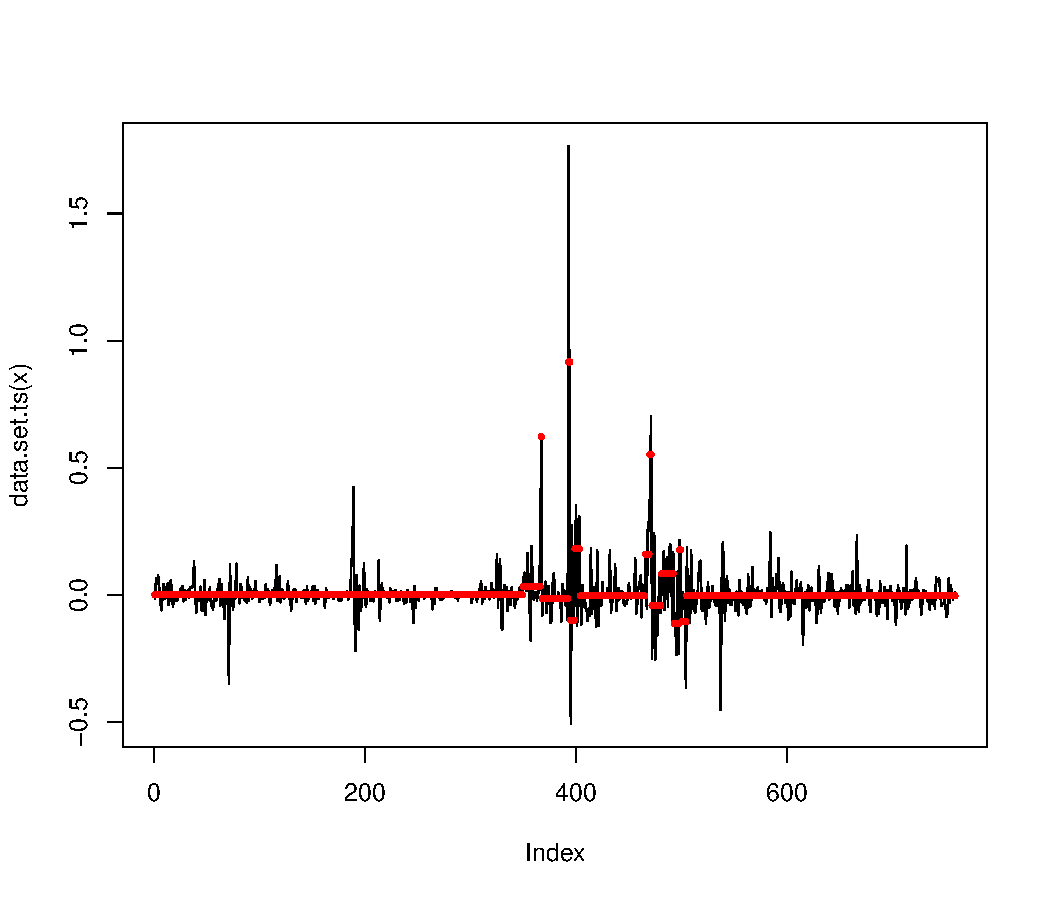
\includegraphics{CopyOfTrial1_files/figure-latex/fig20-1.pdf}
\caption{\label{fig:fig20}Change point in differences of LogDoge}
\end{figure}

The breaking points versus tweet timestamp analysis on Dogecoin currency
confirms and strenghten our findings: there is no trivial linkage
between Musk's tweet and the crypto-currency volatility.

\begin{figure}
\centering
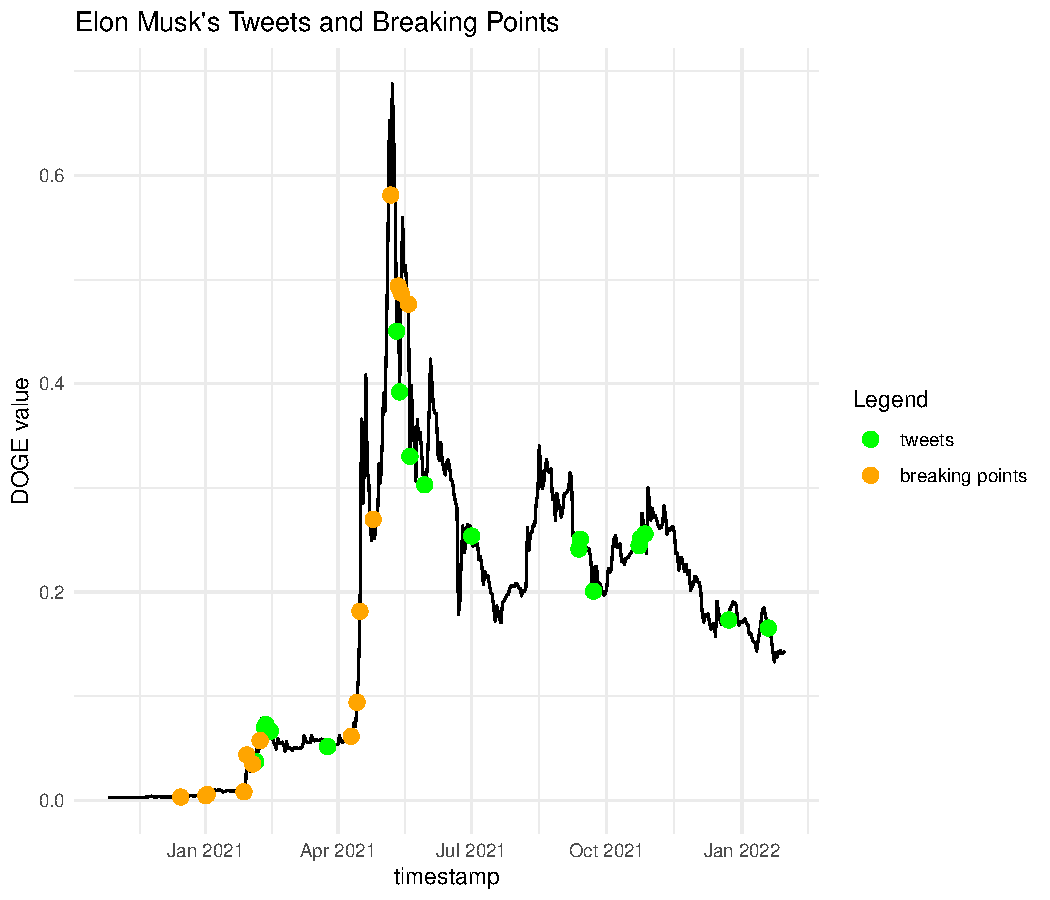
\includegraphics{CopyOfTrial1_files/figure-latex/fig21-1.pdf}
\caption{\label{fig:fig21}Elon Musk's Tweets on Dogecoin and LogDoge's
Changing Points Dates}
\end{figure}

\hypertarget{conclusion}{%
\section{Conclusion}\label{conclusion}}

We have extracted a total of 4787 tweets containing 68676 words from
Elon Musk's twitter profile: we investigate the impact of 26 Twitter
events by Elon Musk on the trading volume and price of the
cryptocurrencies he comments on. Firstly we conducted a popularity
analysis, where the influencing power of the Tesla CEO's can be seen
skyrocketing throughout the years, especially after year 2016. A
sentiment approach has been adopted into investigating his
activity-related emotions, with an overall positive range of emotions
associated to it, as well as a frequency analysis on the most used words
and polarity analysis (Model I). A subset of the focus period has been
investigated in a second model (Model II), namely considering tweets
published from January 2020 and eliminating the most used word in the
Model I (\emph{amp}). Coherent results has been found, with a slight
change in the emotions due to a late-stage of Musk's popularity, with a
more self-conscious, critical and mature audience. Finally, we have
investigated potential linkages between Musk's crypto-related tweets and
Bitcoin volatility comparing \emph{when} those tweets were published to
critical \emph{breaking points} in the currency value: no clear linkage
has been found, assessing the randomness of the Bitcoin trend. Our
result has been similar by applying the same investigation to Dogecoin.

This study contributed to the existing available knowledge on
information aggregation on the internet, particularly by so-called
influencers in social networks. It also serves as a foundation for
assessing the impact of extremely prominent people's views on bitcoin
and financial markets. The findings give market participants a better
foundation for determining the importance of certain tweets. Investors
may use this knowledge to design an alternative investment plan,
regulators could assess the necessity for market intervention, and
influencers could better understand the consequences of their actions on
Twitter.

\hypertarget{annex}{%
\section{Annex}\label{annex}}

\emph{Python code to extract Elon Musks's tweets via Twitter API}

\begin{Shaded}
\begin{Highlighting}[]
\NormalTok{import twint}
\NormalTok{import datetime}

\NormalTok{def }\FunctionTok{delist}\NormalTok{(x)}\SpecialCharTok{:}
\NormalTok{    df }\OtherTok{=}\NormalTok{ x[}\DecValTok{0}\NormalTok{]}
    \ControlFlowTok{for}\NormalTok{ i }\ControlFlowTok{in} \FunctionTok{range}\NormalTok{(}\DecValTok{1}\NormalTok{, }\FunctionTok{len}\NormalTok{(x))}\SpecialCharTok{:}
\NormalTok{        df }\OtherTok{=} \FunctionTok{df.append}\NormalTok{(x[i])}
\NormalTok{    return df}

\NormalTok{def }\FunctionTok{ElonPaginated}\NormalTok{()}\SpecialCharTok{:}
\NormalTok{    data }\OtherTok{=}\NormalTok{ []}
\NormalTok{    start }\OtherTok{=} \FunctionTok{datetime.datetime.strptime}\NormalTok{(}\StringTok{"2011{-}01{-}01"}\NormalTok{, }\StringTok{"\%Y{-}\%m{-}\%d"}\NormalTok{)}
\NormalTok{    end }\OtherTok{=} \FunctionTok{datetime.datetime.strptime}\NormalTok{(}\StringTok{"2022{-}02{-}01"}\NormalTok{, }\StringTok{"\%Y{-}\%m{-}\%d"}\NormalTok{)}
\NormalTok{    date\_generated }\OtherTok{=}\NormalTok{ [start }\SpecialCharTok{+} \FunctionTok{datetime.timedelta}\NormalTok{(}\AttributeTok{days=}\NormalTok{x) }\ControlFlowTok{for}\NormalTok{ x }\ControlFlowTok{in} \FunctionTok{range}\NormalTok{(}\DecValTok{0}\NormalTok{, (end }\SpecialCharTok{{-}}\NormalTok{ start).days)]}
\NormalTok{    date\_generated }\OtherTok{=}\NormalTok{ date\_generated[}\SpecialCharTok{::}\DecValTok{7}\NormalTok{]}
\NormalTok{    date\_generated }\OtherTok{=}\NormalTok{ [}\FunctionTok{date\_obj.strftime}\NormalTok{(}\StringTok{"\%Y{-}\%m{-}\%d"}\NormalTok{) }\ControlFlowTok{for}\NormalTok{ date\_obj }\ControlFlowTok{in}\NormalTok{ date\_generated]}
    \ControlFlowTok{for}\NormalTok{ i }\ControlFlowTok{in} \FunctionTok{range}\NormalTok{(}\DecValTok{0}\NormalTok{, }\FunctionTok{len}\NormalTok{(date\_generated) }\SpecialCharTok{{-}} \DecValTok{1}\NormalTok{)}\SpecialCharTok{:}
\NormalTok{        c }\OtherTok{=} \FunctionTok{twint.Config}\NormalTok{()}
\NormalTok{        c.Username }\OtherTok{=} \StringTok{"elonmusk"}
\NormalTok{        c.Since }\OtherTok{=}\NormalTok{ date\_generated[i]}
\NormalTok{        c.Until }\OtherTok{=}\NormalTok{ date\_generated[i }\SpecialCharTok{+} \DecValTok{1}\NormalTok{]}
\NormalTok{        c.Pandas }\OtherTok{=}\NormalTok{ True}
        \FunctionTok{twint.run.Search}\NormalTok{(c)}
\NormalTok{        Tweets\_df }\OtherTok{=}\NormalTok{ twint.storage.panda.Tweets\_df}
        \ControlFlowTok{if}\NormalTok{ Tweets\_df.empty}\SpecialCharTok{:}
\NormalTok{            pass}
        \ControlFlowTok{else}\SpecialCharTok{:} \FunctionTok{data.append}\NormalTok{((Tweets\_df))}
\NormalTok{    return data}

\NormalTok{data }\OtherTok{=} \FunctionTok{ElonPaginated}\NormalTok{()}
\NormalTok{data }\OtherTok{=} \FunctionTok{delist}\NormalTok{(data)}
\FunctionTok{print}\NormalTok{(data)}
\FunctionTok{data.to\_csv}\NormalTok{(}\StringTok{\textquotesingle{}/Users/federicopiazza/Desktop/MONTREAL/QM/elon.csv\textquotesingle{}}\NormalTok{)}
\end{Highlighting}
\end{Shaded}


\printbibliography

\end{document}
